\documentclass{beamer}
%
% Choose how your presentation looks.
%
% For more themes, color themes and font themes, see:
% http://deic.uab.es/~iblanes/beamer_gallery/index_by_theme.html
%
\mode<presentation>
{
\usetheme{default}      % or try Darmstadt, Madrid, Warsaw, ...
\usecolortheme{beaver} % or try albatross, beaver, crane, ...
\usefonttheme{default}  % or try serif, structurebold, ...
\setbeamertemplate{navigation symbols}{}
\setbeamertemplate{caption}[numbered]
}

\usepackage[portuguese]{babel}
\usepackage[utf8x]{inputenc}
\usepackage{multirow}
\usepackage{ragged2e}
\justifying

\setlength{\parindent}{0.5cm}
%%%%%%%%%%%%%%%%%%%%%
% Títulos e etc
\title[Apresentação Semanal]{Apresentação Semanal}
\author{Miguel Inocêncio}
\institute{Universidade de Aveiro}
\date{26/03/2019}

\begin{document}

%%%%%%%%%%%%%%%%%%%%%
% Página Inicial
\begin{frame}
	\titlepage
\end{frame}

%%%%%%%%%%%%%%%%%%%%%
% Table of Contents
\begin{frame}{Conteúdos}
	\tableofcontents
\end{frame}

%%%%%%%%%%%%%%%%%%%%%%
% Introduções Gerais
\section{HEVC - Introdução Geral}
\begin{frame}{HEVC}
	\begin{itemize}
		\item Projeto lançado em 2010 pela ITU-T Video Coding Experts Group (VCEG) e ISSO/IEC Moving Picture Experts Group (MPEG)
		\item Originou uma nova organização: Joint Collaborative Team on Video Coding (JCT-VC)
		\item Primeira versão lançada em 2013
		\item Sucessor do H.264/AVC
	\end{itemize}

	\begin{figure}
		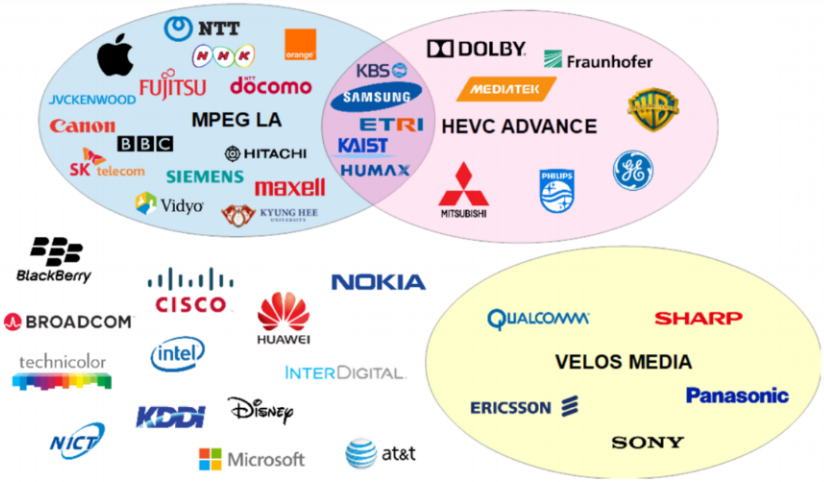
\includegraphics[height=0.4\textheight]{holders.png}
		\caption{\label{fig:hevc_holders}Detentores de patentes do HEVC}
	\end{figure}
\end{frame}

\section{AV1 - Introdução Geral}
\begin{frame}{AV1}
	\begin{itemize}
		\item Formato de compressão Open Source e sem royalties
		\item Finalizada a primeira versão em 2018, pela Alliance for Open Media (AOMedia)
		\item Sucessor do VP9 (formato da Google, usado no Youtube)
		\item Desenvolvido para aplicações de streaming
	\end{itemize}

	\begin{figure}
		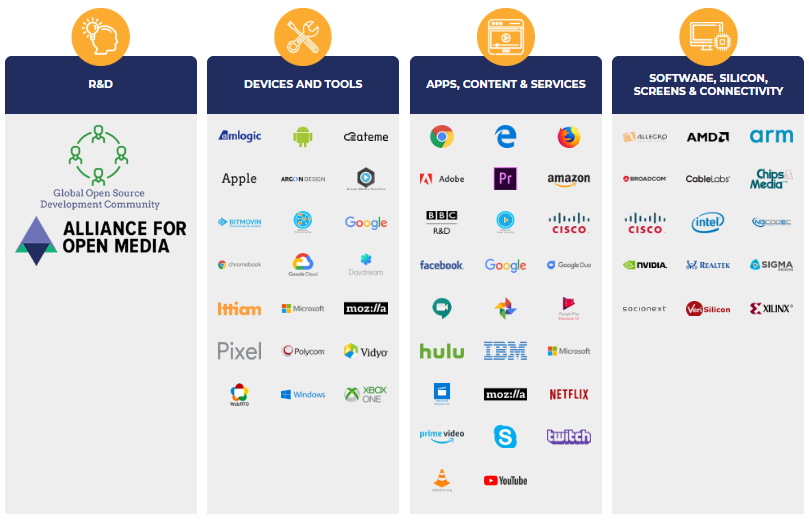
\includegraphics[height=0.5\textheight]{aom.png}
		\caption{\label{fig:AOM}Alliance for Open Media}
	\end{figure}
\end{frame}

%%%%%%%%%%%%%%%%%%%%%
% Comparação Técnica HEVC AV1
\section{Comparação técnica entre HEVC vs AV1}

\begin{frame}{Comparação técnica entre HEVC vs AV1}
	\begin{itemize}
		\item Apresentação geral de ambos os formatos de codificação
		\item Comparação de aspetos técnicos
	\end{itemize}
\end{frame}

\subsection{High Level Syntax}
\begin{frame}{High Level Syntax}
	\begin{table}
		\centering
		\begin{tabular}{l|l|l}
			\textbf{Característica} 					& \textbf{HEVC} 	& \textbf{AV1} \\\hline
			\textbf{Perfis} 									& 14 							& 3 \\
			\textbf{Níveis} 									& 13 							& 12 \\
			\multirow{2}{*}{\textbf{Layers}} 	& Slices 					& Frames divididas \\
			& independentes 	& por Tiles \\
		\end{tabular}
		\caption{\label{tab:high-level}Noções gerais de ambos os codecs}
	\end{table}
\end{frame}

\subsection{Partições}
\begin{frame}{Partições}
	Tamanho máximo \textit{Coding Tree Units}'s no HEVC e \textbf{superblock}'s no AV1, bem como todos os tamanhos usados nas diferentes fases do processo.
	\begin{table}
		\centering
		\begin{tabular}{l|l|l}
			\textbf{Característica} 					& \textbf{HEVC} 	& \textbf{AV1} \\\hline
			\textbf{Nº de tamanhos} 					& 24 							& 42 \\
			\textbf{Tamanho máximo} 					& 64x64 					& 128x128
		\end{tabular}
		\caption{\label{tab:partitioning}Partitioning}
	\end{table}
\end{frame}

\subsection{Intra-Prediction}
\begin{frame}{Intra-Prediction}
	Ambos os formatos usam processos semelhantes, embora o HEVC apenas melhore as tecnologias implementadas no AVC. Neste aspeto, o AV1 adiciona funcionalidades inexistentes no VP9.
	\begin{table}
		\centering
		\begin{tabular}{l|l|l}
			\textbf{Característica} 									& \textbf{HEVC} 	& \textbf{AV1} \\\hline
			\textbf{Nº de modos angulares} 						& 33 							& 56 \\
			\textbf{Nº modos não angulares} 					& 2	 							& 6 \\
			\multirow{2}{*}{\textbf{Outras adições}}	& $\varnothing$		& 5 modos recursivos \\
			&									& 1 \textit{Chroma from Luma} \\
		\end{tabular}
		\caption{\label{tab:intra}Intra-Prediction}
	\end{table}
\end{frame}

\subsection{Inter-Prediction}
\begin{frame}{Inter-Prediction}
	Novamente, ambos os processos seguem abordagens semelhantes. Contudo, o HEVC é mais exigente em termos de memória, enquanto que o AV1 peca pela exigência em termos de complexidade.
	\begin{table}
		\centering
		\begin{tabular}{l|l|l}
			\textbf{Característica} 									& \textbf{HEVC} 	& \textbf{AV1} \\\hline
			\textbf{Nº de modos de predição} 					& 2 							& 4 \\
			\textbf{Nº frames de referência} 					& 8 de 16	 				& 7 de 8 \\
			\multirow{3}{*}{\textbf{Outras adições}}	& $\frac{1}{8} pel$		& Global Motion \\
			&									& 5 filtros de sub-pel \\
			&									& independentes \\
		\end{tabular}
		\caption{\label{tab:inter}Inter-Prediction}
	\end{table}
\end{frame}

\subsection{Transformadas}
\begin{frame}{Transformadas}
	Ambos os formatos manteram as técnicas dos seus predecessores, inovando nos tamanhos dos blocos. Quer isto dizer que o AV1 apresenta um grau de liberdade bastante superior ao HEVC.
	\begin{table}
		\centering
		\begin{tabular}{l|l|l}
			\textbf{Característica} 													& \textbf{HEVC} 	& \textbf{AV1} \\\hline
			\multirow{3}{*}{\textbf{Tipos de transformadas}} 	& DCT e DST 			& DCT, ADST, \\
			&									& Flip ADS e \\
			&									& Identidade \\
			\textbf{Tamanho máximo do bloco} 									& 32x32		 				& 64x64 \\
			\multirow{2}{*}{\textbf{Outras adições}}					& $\varnothing$		& Blocos Retangulares \\
			&									& Blocos Recursivos \\
		\end{tabular}
		\caption{\label{tab:transforms}Transforms}
	\end{table}
\end{frame}

\subsection{Quantização}
\begin{frame}{Quantização}
	Nenhum dos dois formatos sofreu grandes alterações em relação ao análogo anterior. A quantização é feita através de matrizes fixas, que é escolhida a partir de um parâmetro calculado (QP).
	\begin{table}
		\centering
		\begin{tabular}{l|l|l}
			\textbf{Característica} 													& \textbf{HEVC} 	& \textbf{AV1} \\\hline
			\textbf{Nº de parametros para QP}									& 2					 			& 6 \\
			\textbf{Outras adições}														& $\varnothing$		& Offset para superblocos \\
		\end{tabular}
		\caption{\label{tab:quantization}Quantization}
	\end{table}
\end{frame}

\subsection{Codificação de Entropia}
\begin{frame}{Codificação de Entropia}
	Neste ramo, o HEVC retirou um dos modos de codificação, mantendo apenas o CABAC. No caso do AV1, manteve-se a codificação aritmética do VP9, com o aumento do alfabeto.
	\begin{table}
		\centering
		\begin{tabular}{l|l|l}
			\textbf{Característica} 													& \textbf{HEVC} 	& \textbf{AV1} \\\hline
			\multirow{2}{*}{\textbf{Codificação}}							& CABAC			 			& Multi-symbol arithmetic \\
			&									& com alfabeto até 16 \\
			\textbf{Atualização do alfabeto}									& a cada frame		& a cada símbolo \\
		\end{tabular}
		\caption{\label{tab:entropy}Entropy Coding}
	\end{table}
\end{frame}

\subsection{Filtragem}
\begin{frame}{Filtragem}
	Ambos os formatos inovaram neste ramo, adicionando filtros opcionais, assim como formalizando a utilização de filtros opcionais nos formatos anteriores.
	\begin{table}
		\centering
		\begin{tabular}{l|l|l}
			\textbf{Característica} 													& \textbf{HEVC} 	& \textbf{AV1} \\\hline
			\textbf{De-blocking}															& Sim			 				& Sim \\
			\multirow{3}{*}{\textbf{Outros Filtros}}					&	\multirow{2}{*}{Sample Adaptive Offset}	& Constrained Directional \\
			&													&  Enhancement Filter\\
			&													&	Loop Filter \\
		\end{tabular}
		\caption{\label{tab:filtering}Filtering}
	\end{table}
\end{frame}

%%%%%%%%%%%%%%%%%%%%%%%%%%%%
% Comparação de Performance
\section{Análise de Performance}
\begin{frame}{Análise de Performance}
	A performance de ambos os encoders foi avaliada em dois aspetos: qualidade de codificação e tempo de enconding.

	Este último parâmetro está altamente dependente do hardware no qual é implementado, nomeadamente devido à grande maioria das placas gráficas lançadas desde 2016 já possuírem aceleradores de hardware dedicado para encoding/decoding de HEVC. Além disto, também a maturidade dos encoders em software para HEVC e correspondente optimização dos seus processos leva ao aumento da sua vantagem em relação ao AV1.

	Quanto à qualidade objetiva e subjetiva dos formatos, também aqui existe alguma liberdade de resultados, devido aos diferentes perfis a utilizar.
\end{frame}

\begin{frame}{Análise de Performance}
	A complexidade adicional do AV1 é recompensada, devido à qualidade adicional obtida, quando comparada com o HEVC. Contudo, torna-se difícil concluir com um número final, devido à disparidade de resultados encontrada, já que alguns testes mostram acréscimos de 2% em PSNR, enquanto outros mostram 40% de melhorias.

	Quanto ao tempo de codificação, os resultados mais recentes (Julho de 2018) mostram resultados pouco animadores, apesar de terem sido feitas melhorias aos encoders de software posteriormente.

	\begin{table}
		\centering
		\begin{tabular}{l|l|l}
			\textbf{Codificador}		 													& \textbf{Tempo de Encoding (s)} 	& \textbf{x Tempo Real} \\\hline
			\textbf{x265}																			& 289			 												& 58 \\
			\textbf{libaom}																		&	226 080													& 45 216 \\
		\end{tabular}
		\caption{\label{tab:time}Tempo de codificação de clip de 5s}
	\end{table}
\end{frame}

%%%%%%%%%%%%%%%%%%%%%%%%%%%%%
% Documentação
\section{Documentação e Trabalhos Publicados}
\begin{frame}{Documentação}
	Devido à maior longevidade do HEVC, existe mais documentação explicativa, além dos trabalhos publicados pelas equipas de investigação.

	Isto tem também significa que o desenvolvimento de trabalho inovador é difícil de realizar, devido ao grande investimento feito nos ultimos 8 anos neste padrão.

	Quanto ao AV1, este aspecto não se põe em causa. Devido ao quão recente o formato é, os trabalhos publicados são excassos, e muitos apenas representam algumas análises de performance ou revisões bibliográficas.

	Contudo, a excassez de publicações também se verifica no caráter explicativo.

	Apesar disto,a documentação do padrão é bastante clara. Para além do AV1 estar apoiado por empresas que apostam bastante em documentações claras e extensas dos seus projetos Open Source (nomeadamente a Google e Mozilla).
\end{frame}

%%%%%%%%%%%%%%%%%%%%%%%%%%%%%
% Industria
\section{Indústria}
\begin{frame}{Indústria}
	A elevada complexidade de licenseamento do HEVC foi o que levou à criação da \textit{Alliance for Open Media}. Devido aos grandes gigantes da produção de entretenimento estarem neste consórcio, existe uma grande inclinação a uma adoção massiça deste formato.

	Apesar do âmbito da tese de mestrado não ser ir de enconcontro à indústria, o desenvolvimento de trabalho num padrão que tenderá a gerar interesse mundialmente, poderá abrir oportunidades para trabalhos futuros.
\end{frame}

%%%%%%%%%%%%%%%%%%%%%%%%%%%%%
% Conclusão
\section{Conclusões}
\begin{frame}{Conclusões}
	\begin{itemize}
		\item O AV1 apresenta uma complexidade superior ao HEVC em termos do próprio formato, assim como em termos do ambiente de desenvolvimento
		\item Existe um interesse crescente no padrão mais recente
		\item Apesar de recentes, os trabalhos começam agora a surgir devido ao apoio da \textit{AOM}
	\end{itemize}

	Devido à inexperiência em ambos os formatos, bem como no desenvolvimento de trabalhos semelhantes, qualquer que seja a escolha apresentará um desafio semelhante.
\end{frame}

\end{document}
